\usepackage{url}
\title{Predicting financial crises using a recurrent neural network}
\author{
        Pratibha Agarwal \and Dhruvatara Bhogishetty \and Charlie Ann Fornaca \and Angela Rodolico \\
        }

\date{University of California, Davis \\ Fall 2020}

\documentclass[12pt]{article}
\usepackage{graphicx}
\usepackage{float}
\usepackage{incgraph,tikz}

\begin{document}
\maketitle

\begin{abstract}
Our experiment aims to glean insight into predicting the presence of a banking crisis following certain economic parameters and past time series data denoting historical crises. We use deep learning to discover feature representations that one would not naturally be able to detect. The advance that our model would make would provide a layer of economic expectation and financial stability when experiencing national or global crises. This research is particularly pertinent to the current coronavirus crisis at the time of writing this.
\end{abstract}


\section{Introduction}

\subsection{Deep Learning}

Deep Learning is becoming a popular approach to answer some of the unanswered questions in the field of science, economics, commerce etc. In some cases such as banking and science, the results could have direct consequences hence accuracy plays an important role. With the increasing number of DL techniques and algorithms for prediction, size of data, computation time and accuracy play an important role in deciding the model. In the finance sector, DL is being used since a long time for various purposes such as credit card fraud detection, stock market prediction etc. 

\subsection{Financial \& Economic Importance}

It is important for financial institutions to attempt mitigation of a financial crisis.  This importance comes from investors ensuring that their stock investments are worthy and safe. Finding amicable features to predict early onset of global or national economic and banking crisis is no easy feat. There are however a few indications that can be considered notable data points when forming a model such as high inflation of a country's currency\cite{kumar}. 

\subsection{Prior Research}

During our literature review, we came across a work which took African Economic, Banking and Systemic Crisis Data for their experiment. This is the data on the economic and financial crisis in 13 African countries between 1869 to 2014. This dataset contains 14 attributes of 1060 observations and the last attribute in the dataset contains categorical values which shows if the crisis took place or not. They designed an ANN model for the prediction using their data. 

\section{Methods}
\subsection{Data \& Data Cleaning}
Our data came from Harvard Business School’s Behavioral Financial & Financial Stability’s Global Crisis Data by Country dataset \cite{harvard}. We also used unemployment rate data provided by the Federal Reserve Bank of St. Louis \cite{fred}.The gross domestic product and GDP per capita data came from the collection of the late Professor Angus Maddison of the University of Groningen’s Grogningen’s Growth & Development Centre \cite{ggdc}.

There were several factors that we used to contribute to our prediction model represented as columns in our dataset. Those columns are described below.

We considered three North American countries to build our prediction model: Canada, Mexico, and the United States. We also included the year in which each data point was from as it was an indicator later on whether the country was in fact a country (as opposed to a colony for some of the older data entries). 
Another feature is whether the country’s currency within that particular year followed the gold standard. Gold standard indicates whether a currency under the country’s government is fixed to and may be freely exchanged or converted to gold or bank notes worth gold \cite{chengold}.

A column indicating presence of domestic debt is also included. According to National Bureau of Economic Research (NBER) scholars, Reinhart and Rogoff, “domestic debt is often much larger than the monetary base in the run-up to high-inflation” \cite{nber}. We surmise that this column would be valuable in its contribution to predicting an economic crisis. Another debt-measure, sovereign debt, is used in this dataset. Sovereign or government dept, is the central government's debt. It is usually issued by the government from foreign currency for financing growth and development \cite{chensovereign}.

Self-explanatory economic related columns that were also considered included an exchange rate in comparison to the United States dollar, gross domestic product (GDP), weighted default GDP, inflation in regards to annual percentages of average consumer prices, and annual unemployment rate. 

Finally, the column in which we aimed to predict was the “Crisis” column. This was a simple 1 or 0 that indicated the presence of a recorded crisis for the year and country of the row it resides in.

Before moving onto building models, we realized that we also had to discard data from before the year 1899. Canada and Mexico were not considered countries in the same way that the United States had gained independence and instead had regions considered colonies under various European powers at the time. Because of this, we had missing data and ultimately decided to drop rows from before the twentieth century. A column that was also an indicator of this status in data after 1899 that was retained, was the independence column. This column was another binary 0 or 1 that denoted if the country was presently independent or not.

\subsection{Creating a Baseline Logistic Regression Model}
After cleaning and preparing the dataset, we created a baseline logistic regression model to predict the presence of a crisis indicator (0 or 1). When creating the model we ended up dropping the country column as it wasn’t quantitative data and also we didn’t want to take the specific country into account for our prediction. We also dropped a column describing the GDP per capita. We decided to use logistic regression because of its simplicity as a classifier in order to develop our baseline model. In the model, we have an input layer, whose output was further embedded and the embedding was supplied to the LSTM layer whose output is supplied to the Dense layer which is our last layer. The architecture can be explained using the following diagram:\\
\begin{center}
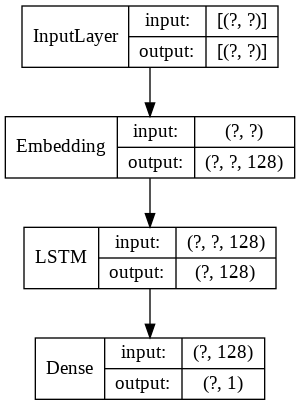
\includegraphics[scale=0.5]{model_3(1).png}\\
\end{center}



\section{Results}
\subsection{Basic LSTM Model}
Economic crises bare a cyclical nature \cite{10.1007/978-3-030-15577-3_11}. Hence, we decided to train our neural network with an LSTM layer. With numeric values in the data set ranging from -20.965125073082 to 9485136.0, we have a very big input dimension. In order to shrink the input dimension, We employed an embedding layer to reduce the input dimension to 32. However, since the embedding layer only accepts positive values, we first tested the feasibility of our model without data from the "Inflation, Annual percentages of average consumer prices column". The input then goes to an LSTM layer for training. We obtained a training accuracy of 53.31\%.

Baring in mind that this accuracy is low, we hypothesized that data from the "Inflation, Annual percentages of average consumer prices" column may still hold its importance in training the neural network. Therefore, in order to preserve the scale of the data and difference between series, we attempted to normalize the data by adding the absolute value of the lowest value in the column to each value in that same column. We trained the LSTM again with the newly modified data frame. However, the training accuracy decreased further to 25.65\%. Other avenues to correctly exercise the importance of this feature needs to be explored. 

\subsection{Improved LSTM Model}
Firstly, we decided to tackle with the issue of normalization. This time, instead of modifying the values of one single column, we implemented MinMaxScaler and normalized values of the entire dataset.

Secondly, we added a validation split to better train the hyperparameters of the model. It can be noted that our validation loss was more elevated than our training loss. Since we have a small training dataset (232 rows), it could cause our model to overfit. In order to mitigate the issue, we added a validation split of 0.1 when training the model. This helped reduce the difference between training and validation loss.

Thirdly, after switching from binary cross entropy to mean squared error, the training loss also reduced.

Fourthly, we then investigated our activation functions. We decided that merely employing sigmoid activation in both the LSTM and dense layers would neglect a good portion of important data within the neural network and cause the activation to be overly selective. Therefore, for the LSTM layer, we changed the activation to tanh and recurrent activation to relu. However, we left the activation function as sigmoid in the dense layer since our model addresses the binary classification problem of predicting a financial crisis. 

As figure 2 suggests, with 32 units in the LSTM layer, training and validation accuracy vary little between the model constructed with tanh activation and sigmoid activation. However, in figure 3, we can see that the loss is significantly lower for the tanh activated model(training loss: 16.77\%, validation loss: 23.70\% as opposed to a 51.73\% training loss and 62.68\% validation loss of the sigmoid activated LSTM model).

Finally, for the output dimension of the embedding layer, after having experimented with 32, 64, 128, and 256 dimensions(figure 2 and 3), we deduced that an output dimension of 128 in this layer yields the least loss for both training and validation loss. Moreover, it also generates the highest training and validation accuracy. 

With all 5 modifications mentioned above, we trained our model 300 times and obtained a training loss of 16.85\%, training accuracy of 78.37\%, validation loss of 21.75\%, and validation accuracy of 70.83\%

\newpage
\begin{figure}[H]
    \centering
    \incgraph[documentpaper]
  [width=\paperwidth,height=0.9\paperheight]{accuracy_history.png}
    \caption{Accuracy History}
\end{figure}

\newpage
\begin{figure}[H]
    \centering
    \incgraph[documentpaper]
  [width=\paperwidth,height=0.9\paperheight]{loss_history.png}
    \caption{Loss History}
\end{figure}

\newpage
\section{Discussion}
For our project, we decided to implement RNN to predict the financial crisis for a country. We started with a small Neural Network with 12 input dimensions and 64 output dimensions and an LSTM and dense layer. We failed to get a high accuracy as our data was not normalized and there were both positive and negative set of values. We then normalized our data using sklearn's \textit{MinMaxScaler} which normalized our dataset translating each feature between zero and one. This induced uniformity in the dataset and the model started performing better. We used Canada and USA for training purposes and Mexico's data for testing. We then started playing around with the RNN and its layers. We chose our input dimension as 2 and output dimension as 128. \textit{Tanh} being the default was chosen as the activation function and as for the recurrent activation function, \textit{relu} worked the best for us, also because of the reason that we did not have any negative values after normalization. One of the biggest influencing factors that helped us reduce our loss was changing the loss function. We decided to change it from Binary Cross Entropy to \textit{Mean Squared Error}. Even though generally Binary Cross Entropy works better than MSE for classification data \cite{Shiva:2019}, we were quite surprised how our model performed differently. This hugely affected our loss and thus increased our accuracy.\\
One of the reasons for our low accuracy we feel could be the less data for training our model. We decided to train with model only for the twentieth century because of the limited availability of data for all the three countries and for all the features. We feel training with more data could improve our accuracy.\\
Following is the confusion matrix for our model: \\
\begin{center}
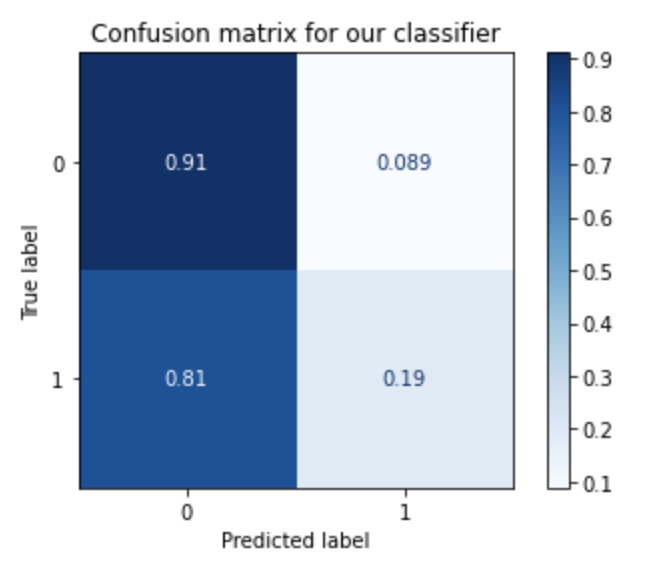
\includegraphics[scale=0.8]{ConfusionMatrix.png}\\
\end{center}
Here, as we can see that the model predicts 0 (i.e. no crisis) with 91\% accuracy but 1 (i.e. crisis) with only 19\% accuracy. This can be justified by the fact that our dataset has a lot more zeros than ones hence it is easier for the model to classify as 'no crisis'. Also in the case of false negatives and false positives, it is easier for the model to predict a false negative because of the large number of 'no crisis' data.\\
With all the changes and tweaks to our initial model, we were able to predict the financial crisis with an accuracy of \textbf{\textit{78.37\%}}.

\section{Author Contributions}
Most of the coding that was performed in this project was done in a peer setting. While one person typed, the other group members(s) helped catch errors and provide feedback. Zoom screen share was heavily utilised to create this partnership between group members. With that being said, here are a few more specific breakdowns as requested in the project guide. 

Angela found the initial dataset that inspired our research. Dhruvatara managed our Github repository and enabled us to easily work together and save our progress through our project. Charlie did the initial data cleaning and notebook set-up. Pratibha and Angela stitched together additional datasets. Dhruvatara refined the dataset afterwards and prepared it for modeling alongside Charlie. Dhruvatara also created the baseline logistic regression model. Pratibha and Angela worked on the recurrent neural network with Charlie involved for feedback. Dhruvtara normalized the data with MinMaxScaling and modified the LSTM model. Angela refined the RNN to get the final training/validation accuracy/loss and made financial crisis prediction with the model. Angela wrote the Results section of the paper. Charlie wrote the Abstract, Introduction, and Methods sections. Pratibha also wrote subparts of the Introduction and Methods sections. Pratibha worked on the Discussion section and the confusion matrix for the model. 

\bibliographystyle{unsrt}
\bibliography{bibliography}
\printbibliography

\end{document}
